%************************************************
\chapter{Reflective Symbolization}
\label{chapter:reflective_symbolization}
%************************************************

\section{Representing Reflective Thinking Activity}

Reflective thinking exists as activities in Duration alongside the
physical activities that have just been described.  I will refer to
the subgraph of the simulation state, $S$, that represents the
$\text{reflective}^1$ thinking activities as $\mathcal{R}^1$.  The
first symbolic references to reflective thinking are now introduced to
this layer of the model.  Note that I have not introduced any specific
symbolic physical activity to the model.  The block example is just
that, an example.  Having no required specific symbolic references in
the physical layer of the description of the general reflective
simulation is important for keeping the representation for the
reflective focus as any labelled graph, which subsequently allows for
reflection over itself, whatever the specific graph representation of
reflective thinking that will now be described.  This is a key point
because the fact that the general model of reflection applies to
\emph{any} given labelled graph means that it allows for this
recursive definition of layered reflective thinking.

\section{Physical Activity is Any Prior Existing Graph}

The graph of physical activities must necessarily exist prior to
reflectively thinking about it.  Because this prior activity is
defined to be \emph{any} graph, what remains in order to build $n$
layers of reflective thinking activity is to define a reflective
planning activity that reflects upon this prior activity.  Therefore,
subsequently, no matter what the reflective thinking description, this
reflective thinking activity can be duplicated in $n$ reflective
layers that will reflectively think about any given graph
representation of activity.  Allowing the physical activity to a be an
undescribed graph is important in order to allow this recursion.
Notice that the physical activity is not necessarily composed of
anything resembling objects as graphs are a very general
representation that could just as easily represent one single number
line, or even an infinitely finely interpolated multidimensional
Space.  If some prior physical activity can be represented as a graph,
then this simulation of reflective thinking is applicable.

\section{Defining N Layers of Reflective Thinking Activities}

Layers of reflective activity are defined inductively, beginning with
$\text{reflective}^0$ layer of activity, $\mathcal{R}^0$, as the
initial given physical activity, $\mathcal{P}$.  Then, each subsequent
layer of $\text{reflective}^{n+1}$ thinking activity,
$\mathcal{R}^{n+1}$, is defined in terms of $\mathcal{R}^n$ in
{\mbox{Equations~\ref{equation:define_reflective_n_activity_graph_first}}}
{\mbox{through~\ref{equation:define_reflective_n_activity_graph_last}}}.
\begin{align}
\label{equation:define_reflective_n_activity_graph_first}
                                        \mathcal{R}^0 &= \mathcal{P} \\
                                   \mathcal{R}^{n+1}_V &\subset S_V \setminus \bigcup_{k=0}^n\mathcal{R}^k_V \\
                                   \mathcal{R}^{n+1}_E &= (\mathcal{R}^{n+1}_V \times \mathcal{R}^{n+1}_V) \cap S_E \\
\label{equation:define_reflective_n_activity_graph_last}
                              \mathcal{R}^{n+1}_\mu(e) &= {\left\{
                                                            \begin{array}{ll}
                                                              S_\mu(e)          & \text{if }e {\in} \mathcal{R}^{n+1}_E \\
                                                              \text{undefined} & \text{otherwise}
                                                            \end{array}
                                                          \right.}
\end{align}
Note that there can be edges between activities in subsequent layers.
These edges are not within any of the graphs of the reflective layers
of thinking, but they do exist in the state graph, $S$.  The edges
that relate the reflective layers of activity in the simulation model
are a necessary component of dynamic symbolic references to activities
in the layers below the symbolic activity.  In other words,
$\bigcup_{k=0}^\infty\mathcal{R}^k\ \subset\ S$, the simulation state
is greater than the union of its reflective layers.

\section{Representing a Graph in the State}

The most important aspect of the reflective simulation is the
capability to create a static reference, $x^*$, to a dynamic
reflective representation of an arbitrary subgraph of activity,
$\Psi(x^*)$, in the layers below the static reference.  Because the
simulation state is a static symbolic representation of the actual
dynamic activities in Duration, simulation of the dynamic reflective
representation must also be in the same simulated terms of dynamic
physical activities.  Considering this dynamic activity to be symbolic
helps in explaining the relationship between the dynamic and the
static, as long as the distinction is kept clear and the simulation of
the dynamic is not confused with the simulation of the static.  The
confusion would arise because both are modelled as symbols in the
state graph, $S$, of the simulation model.  Of course, in actuality,
the dynamic physical activities do not have symbolic terms.  I will
continue to use the asterisk (*) notation when referring to the
simulation of actively static symbolic references as opposed to the
simulation of the otherwise purely dynamic activities in Duration.
{\mbox{Equations~\ref{equation:first_order_reflection_representation_in_state_first}}}
{\mbox{through~\ref{equation:first_order_reflection_representation_in_state_last}}}
show a definition of a static symbolic reference, $x^*$, to a dynamic
reflective representation of a subgraph of activity, $\Psi(x^*)$, all
within the state graph, $S$.
\begin{align}
\label{equation:first_order_reflection_representation_in_state_first}
                                                                    \Psi(x^*) &\subset S \\
                                                         x^*.\text{\tt{node}} &= \Psi_V(x^*) \\
                                               \forall e \in \Psi_E(x^*), x^*_e &\in x^*.\text{\tt{edge}} \\
   \forall_{e \in \Psi_E(x^*)}, e = (e_{v_1}, e_{v_2}) \wedge x^*_e.\text{\tt{tail}} &= \{e_{v_1}\} \\
   \forall_{e \in \Psi_E(x^*)}, e = (e_{v_1}, e_{v_2}) \wedge x^*_e.\text{\tt{head}} &= \{e_{v_2}\} \\
\label{equation:first_order_reflection_representation_in_state_last}
                              \forall_{e \in \Psi_E(x^*)}, x^*_e.\text{\tt{label}} &= \Psi_\rho(x^*)(e)
\end{align}

\section{Representing the Reflective Focus}

Once there is given physical activity defined in the state graph, $S$,
the first-order reflective activity is a dynamic reference to this
given activity.  Here, I introduce the first symbolic references to
this dynamic first-order reflective activity,
$\text{\tt{reflective}}^{n*}$.
{\mbox{Equations~\ref{equation:reflective_symbol_in_state_first}}}
{\mbox{and~\ref{equation:reflective_symbol_in_state_last}}} define the
reflective focus on the given activity.
\begin{align}
\label{equation:reflective_symbol_in_state_first}
      \text{\tt{reflective}}^{n*} &\in \mathcal{R}^n_V, \text{~for $n \geq 1$} \\
\label{equation:reflective_symbol_in_state_last}
\Psi(\text{\tt{reflective}}^{n*}) &\subset S \setminus \bigcup_{k=n}^\infty\mathcal{R}^k_V
\end{align}
{\mbox{\autoref{figure:simulation_reflective_1_example_state}}} shows
how the $\text{\tt reflective}^{1*}$ symbol* activity is in a
continuous dynamic Spatial arrangement with the physical layer of
activities.
\begin{figure}
\center
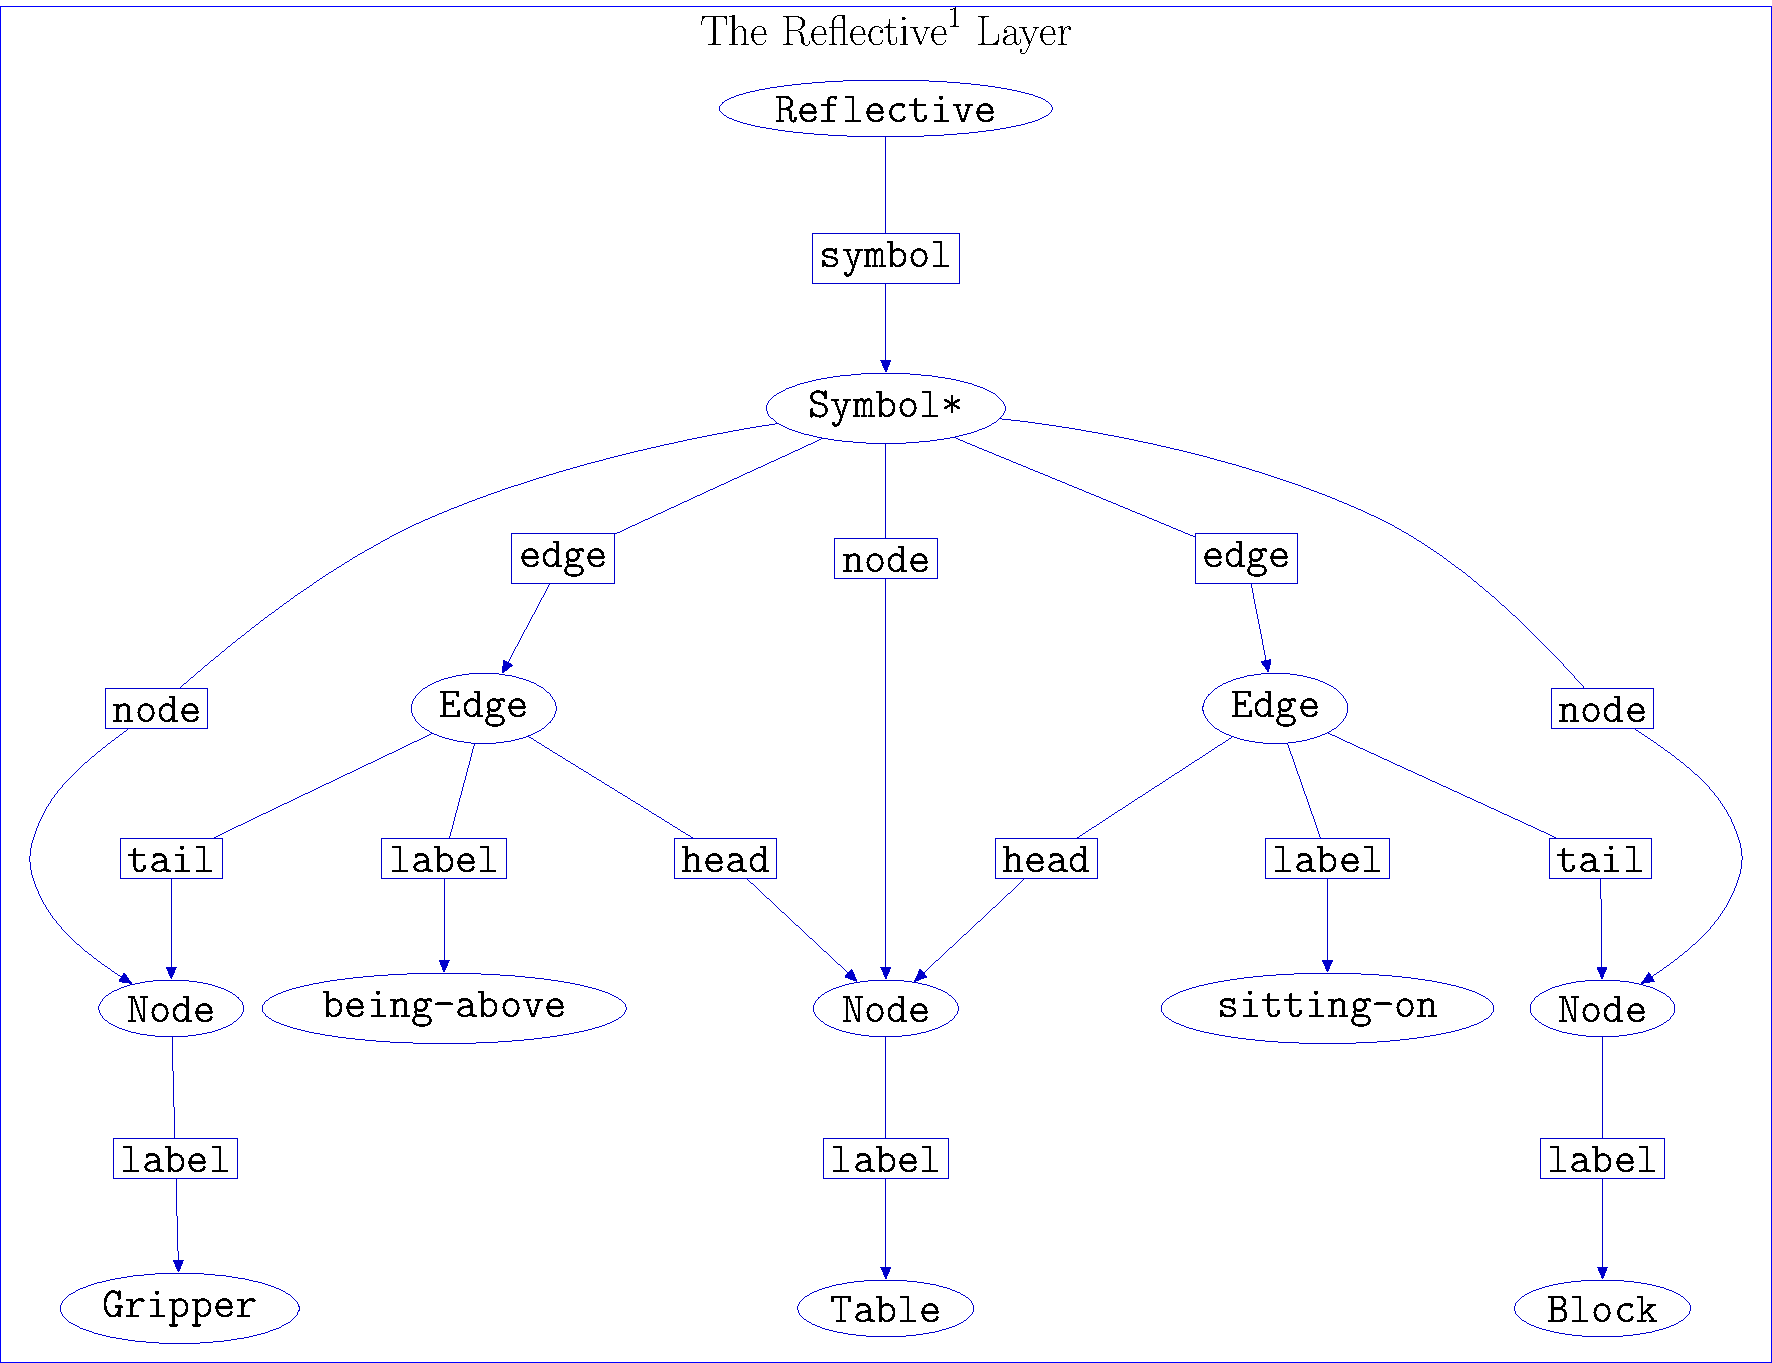
\includegraphics[width=12cm]{gfx/simulation_reflective_1_example_state}
\caption[The static symbolic $\text{\tt reflective}^{1*}$ activity
  focused on the $\text{reflective}^0$ layer of purely dynamic
  activities.]{The static symbolic $\text{\tt reflective}^{1*}$
  activity focused on the $\text{reflective}^0$ layer of purely
  dynamic activities, where black and blue colors distinguish
  $\text{reflective}^0$ and $\text{reflective}^1$ layers of Spatial
  arrangements of activities, respectively.  Note that the red, dashed
  lines represent those Spatial arrangements that are in the
  simulation state, $S$, but are not contained within any specific
  reflective layer of activity.}
\label{figure:simulation_reflective_1_example_state}
\end{figure}

\section{A Visualization of a Reflective Relationship}

When reflective graph structures, as in
{\mbox{\autoref{figure:simulation_reflective_1_example_state}}}, get
to be larger, they can be confusing when shown in full structural
detail.  In order to simplify the visual representation of a
reflective relationship, I will sometimes use a trapezoidal edge-like
visual in order to present the same complicated relationship structure
in a simpler way.
{\mbox{\autoref{figure:reflective_relationship_visualization}}} shows
a simpler visualization of the same example reflective relationship.
\begin{figure}
\center
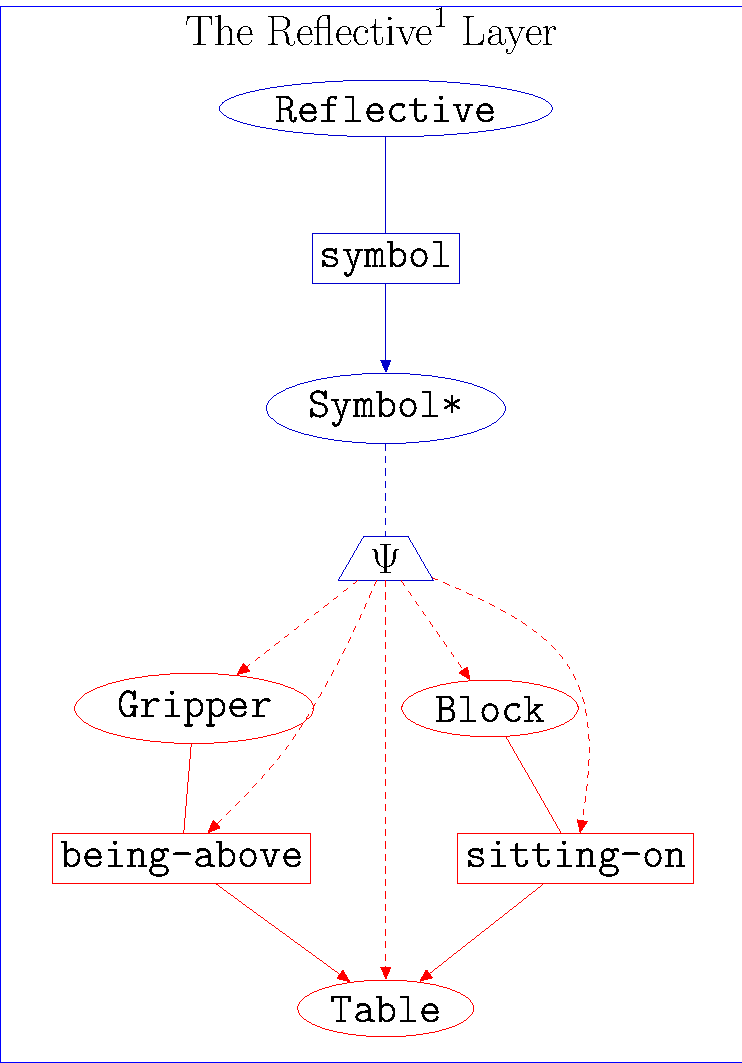
\includegraphics[width=8cm]{gfx/reflective_relationship_visualization}
\caption[A reflective relationship visualization.]{A reflective
  relationship visualization, where the trapezoid is a visual
  representation, a shorthand, for the same reflective relationship
  depicted in
  {\mbox{\autoref{figure:simulation_reflective_1_example_state}}}.
  Thus, the reflective reference operator, $\Psi$, is not a symbol in
  the state graph, $S$.}
\label{figure:reflective_relationship_visualization}
\end{figure}

\section{Representing Symbolic Reference}

In order to describe symbolization, a representation for a simulated
symbol must be defined.  A symbol is the most interesting object in
the model because it functions as a static reference to the dynamic,
while being fundamentally dynamic itself.  There are two primary
features of a symbolic reference:
\begin{itemize}
\item A symbol functions as a static reference and, thus, can be
  ordered in Spatial arrangements that function as static orderings.
\item A symbol is fundamentally dynamic and, thus, exists as dynamic
  activities in a referential dynamic continuous Spatial relationship
  with other dynamic activities in Duration.
\end{itemize}
A symbol is actively maintained in Duration, so the existence of a
simulated symbol in the simulation model would need to be added to the
set of all simulated activities in Duration.  The set of symbols* in
layer $n$ is defined to be $X^{*n}$.
{\mbox{Equations~\ref{equation:define_symbol_first}}}
{\mbox{and~\ref{equation:define_symbol_last}}} define layered sets of
symbols*:
\begin{align}
\label{equation:define_symbol_first}
           X^{*n} &= \text{\tt{reflective}}^n.\text{\tt{symbol}} \\
\label{equation:define_symbol_last}
           x^{*n} &\in X^{*n}
\end{align}
Each symbol*, $x^{*n}$, has a reflective focus, $\Psi(x^{*n})$, a
subgraph of the simulated activities in Duration, $S$.
{\mbox{Equation~\ref{equation:define_symbol_referent_graph}}} defines
the referent subgraph, $\Psi(x^{*n})$, for a symbol*, $x^{*n}$:
\begin{equation}
\label{equation:define_symbol_referent_graph}
  \Psi(x^{*n}) \subseteq X^{*n} \cup \bigcup_{k=0}^{n-1}\mathcal{R}^k_V
\end{equation}

\section{Representing Symbolic Perception and Memory}

{\mbox{\autoref{figure:example_symbolic_reference_to_physical_activity}}}
shows an example of a symbol*, $x_1^*$, in the first-order reflective
layer.  Notice that $\Psi(x_1^*)$ is a subgraph of
$\Psi(\text{\tt{reflective}}^1)$.  When a symbolic reflective
reference is contained within the reflective focus, the symbol is said
to be a \emph{symbolic perception}, or simply, a \emph{percept}.
{\mbox{\autoref{equation:definition_of_symbolic_percept}}} defines
when a symbolic referent is considered a percept based on its
containment relationship with the reflective focus:
\begin{equation}
\label{equation:definition_of_symbolic_percept}
\text{percept}(x_1^*) \longleftrightarrow [\Psi(x_1^*) \subseteq \Psi(\text{\tt{reflective}}^1) \wedge \Psi(x_1^*) \neq \emptyset]
\end{equation}
{\mbox{\autoref{figure:example_symbolic_memory}}} shows a symbolic
reflective reference, $x_2^*$, to the physical layer of activity that
is not perceived because it is not contained within the first-order
reflective focus.  When a symbol is not contained within the
reflective focus, this is referred to as a \emph{symbolic memory}.
Note that the physical, $\text{reflective}^0$ layer of activity
includes all physical activity, including not only current symbolic
perceptions but also symbolic memories.  In this sense, as the AI
changes reflective focus, the perceived dynamic physical activity
changes.
\begin{figure}
\center
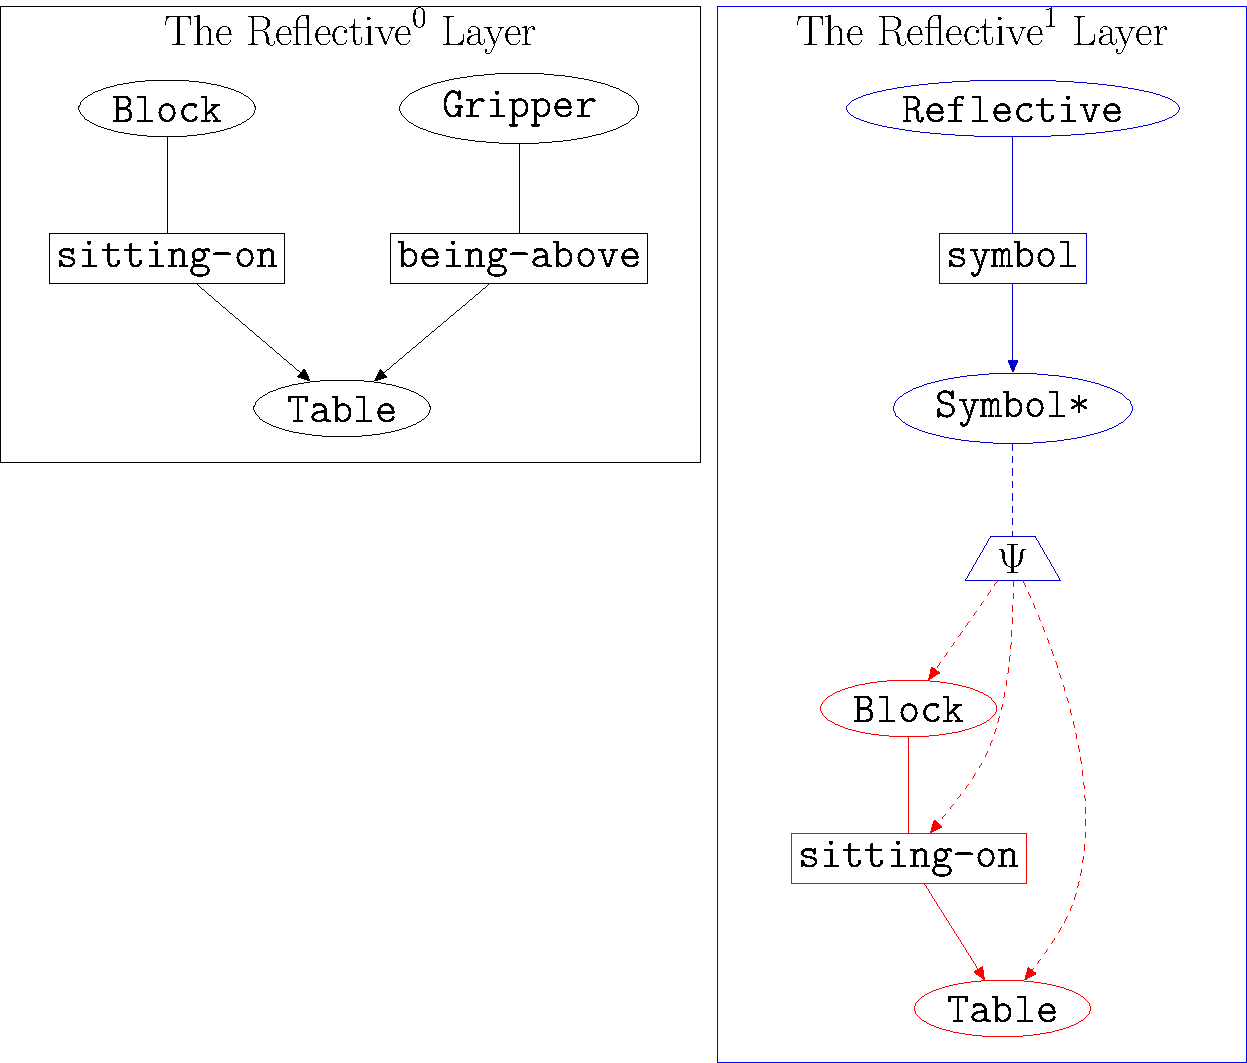
\includegraphics[height=10cm]{gfx/example_symbolic_reference_to_physical_activity}
\caption[Example of a perceived first-order symbolic reference to the
  physical layer of activity.]{Example of a perceived first-order
  symbolic reference, $x_1^*$, to the physical layer of activity,
  i.e. $\Psi(x_1^*)\subseteq\Psi(\text{\tt{reflective}}^1)$.}
\label{figure:example_symbolic_reference_to_physical_activity}
\end{figure}
\begin{figure}
\center
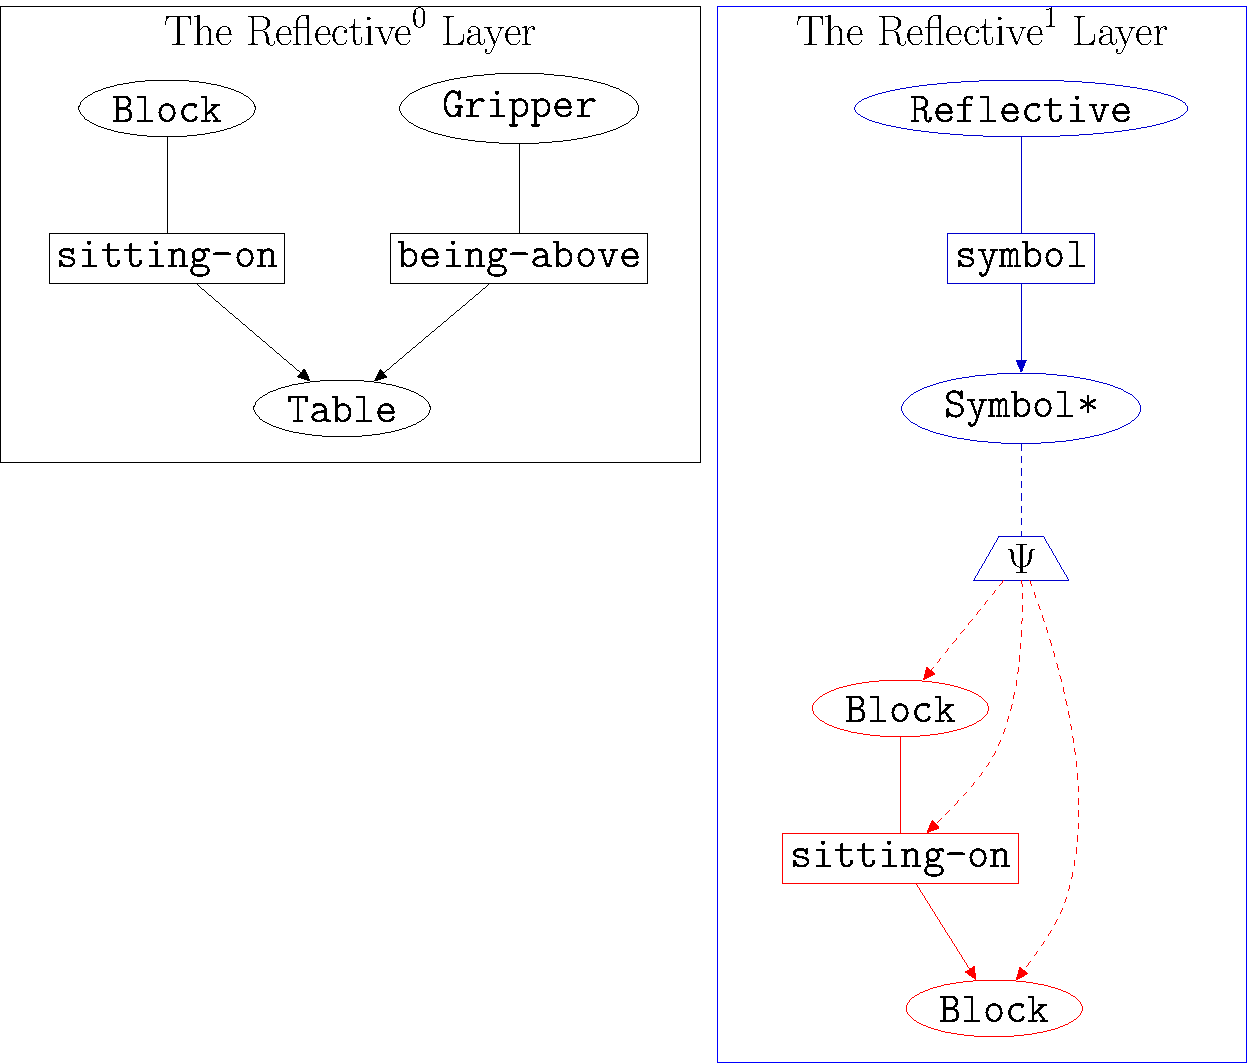
\includegraphics[height=10cm]{gfx/example_symbolic_memory}
\caption[Example of a non-perceived symbol, or symbolic
  memory.]{Example of a non-perceived symbol, or symbolic memory,
  $x_2^*$,
  i.e. $\Psi(x_2^*)\not\subseteq\Psi(\text{\tt{reflective}}^1)$.}
\label{figure:example_symbolic_memory}
\end{figure}


